
\chapter{Mach waves, shock waves and Prandtl-Meyer expansion}
\section{Weak solutions of the flow equations}
	Flow equations also allow non-continuous solutions $\rightarrow$ \textbf{weak}. We limit the study to stationary weak solutions for which the discontinuity does not change in time. We restrict ourselves to non viscous 2D flows, respecting Euler equations (mass, momentum, energy) which allows discontinuities. Let's remind the Euler hyperbolic equation and the scalar convection equation: 
	
	\begin{equation}
	\frac{\D u}{\D t} + a \frac{\D u}{\D x} = 0 \qquad u = f(x-at) = f(q)
	\end{equation}
	
	The derivatives give: 
	
	\begin{equation}
	\frac{\D u}{\D t} = \frac{\D f}{\D q} \frac{\D q}{\D t} = \frac{\D f}{\D q} (-a)\qquad \frac{\D u}{\D x} = \frac{\D f}{\D q} \frac{\D q}{\D x} = \frac{\D f}{\D q} (1)
	\end{equation}
	
	\begin{center}
	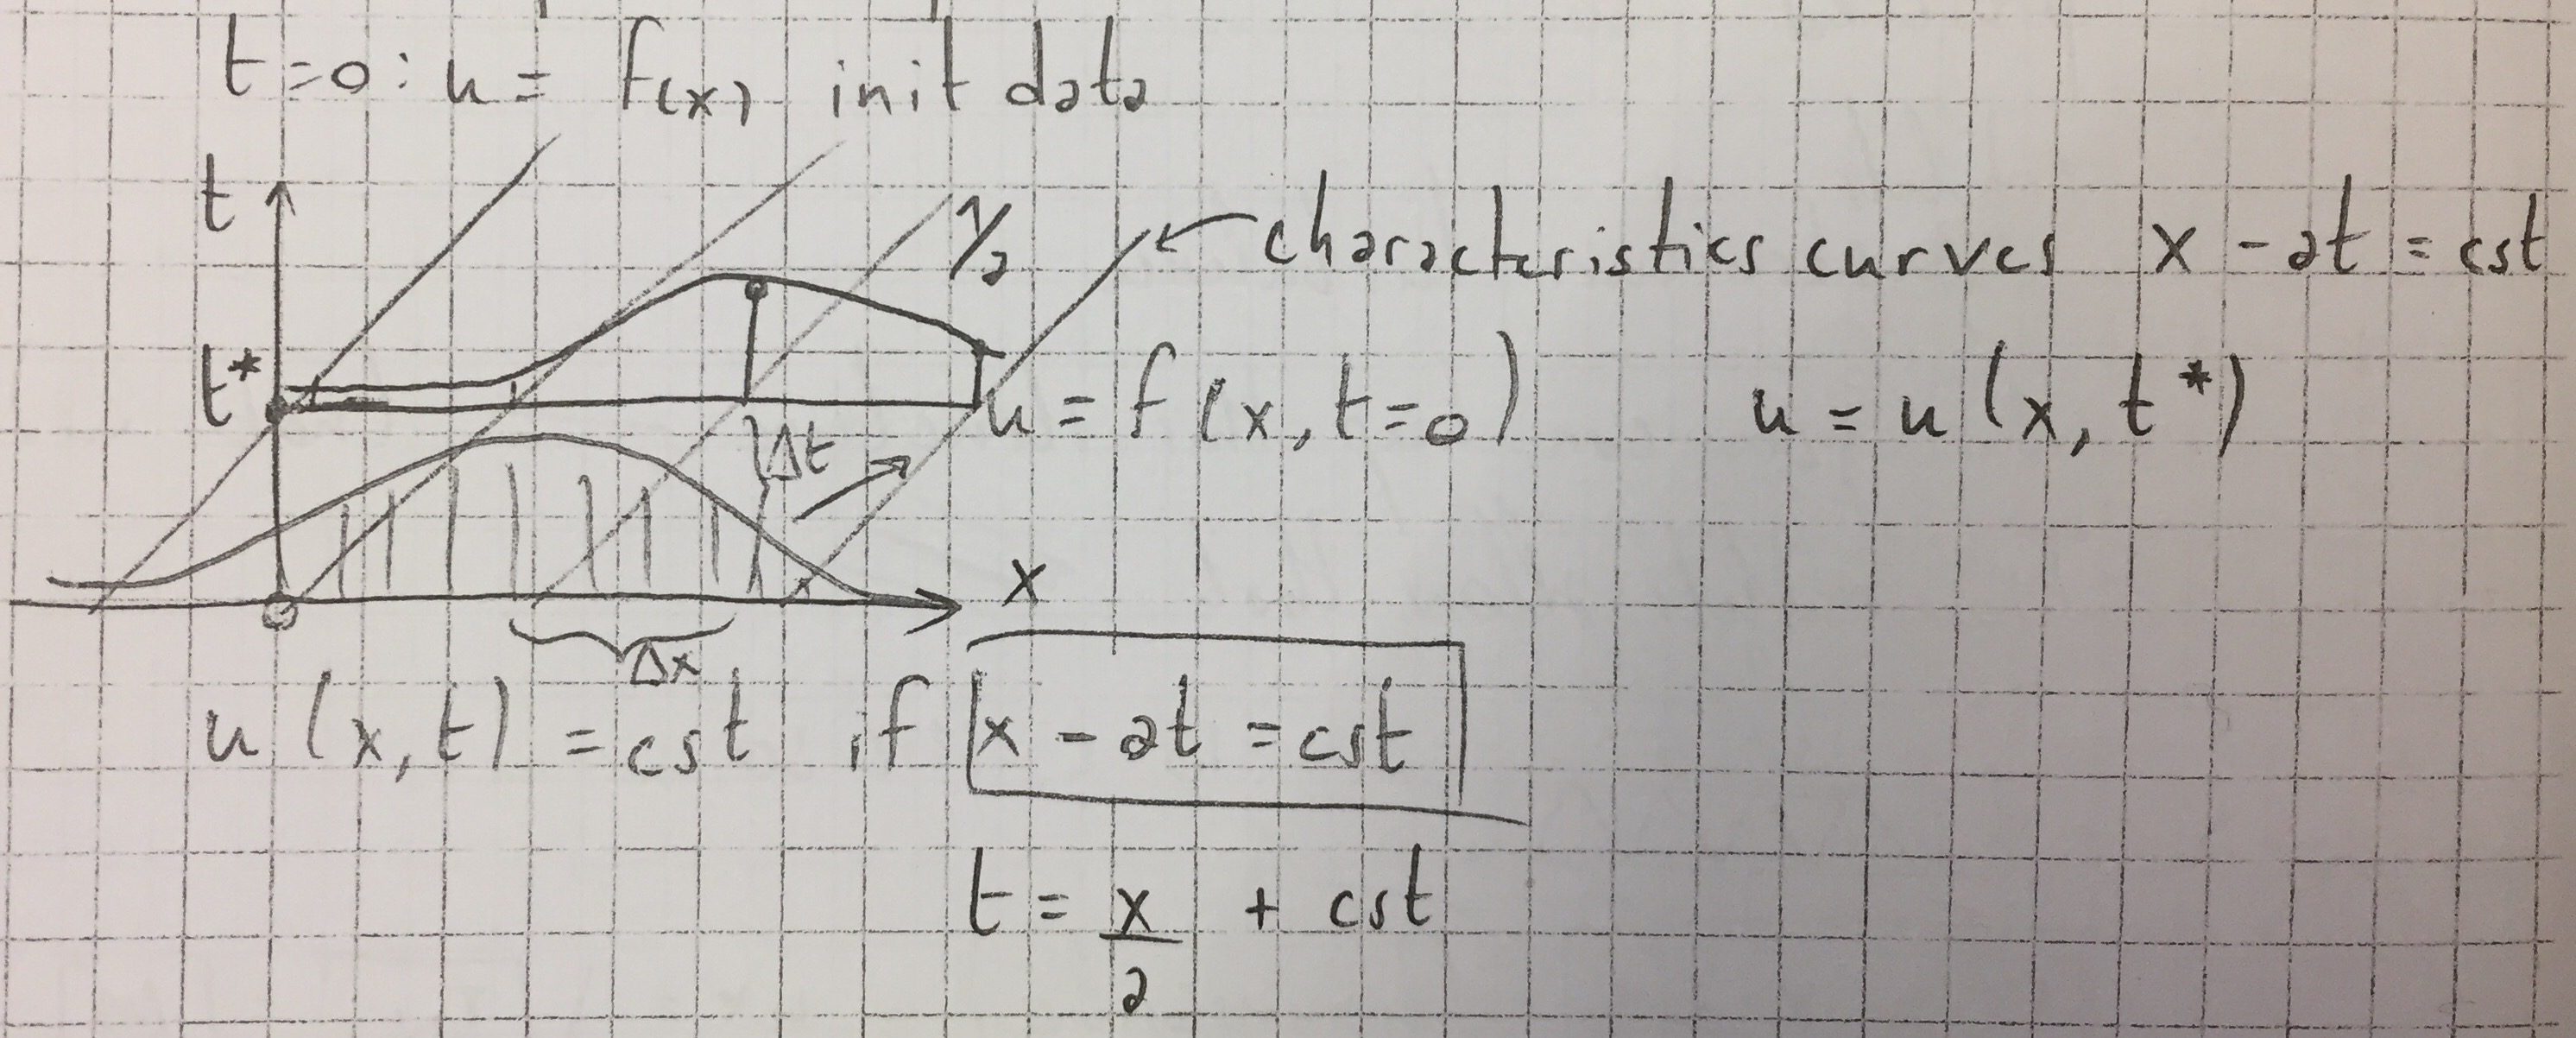
\includegraphics[scale=0.1]{ch8/7}
	\captionof{figure}{}
	\end{center}
	
	Initial wave is shifted on the right. Euler equation in 2D comes from the 1D momentum equation: 
	
	\begin{equation}
	\frac{\D u}{\D t} + u\frac{\D u}{\D x} = \frac{1}{\rho } \mu \frac{\D u^2}{\D  x^2} + \cancel{\frac{1}{\rho }\frac{\D p}{\D x}}
	\end{equation}
	
	Ir the Re number tends to infinity, the right side is canceled and we switch from N-S equations to Euler equation:
	
	\begin{equation}
	\begin{array}{c}
	\frac{\D u}{\D t} + \frac{\D F}{\D x} + \frac{\D G}{\D y} = 0 \\
	u= \left( \begin{array}{c}
	\rho \\
	\rho u\\
	\rho v\\
	\rho E
	\end{array}
	\right)
	\qquad 
	F= \left( \begin{array}{c}
	\rho \\
	\rho u^2 + p\\
	\rho uv\\
	\rho uH
	\end{array}
	\right)
	\qquad 
	u= \left( \begin{array}{c}
	\rho v\\
	\rho uv\\
	\rho v^2 +p\\
	\rho vH
	\end{array}
	\right)
	\end{array}
	\end{equation}
	
	where u is the vector of \textbf{conservative variables}, F and G are the \textbf{flux vectors}, E the total energy and H the total enthalpy. More compact: 
	
	\begin{equation}
	\frac{\D  u}{\D t} + \nabla \bar{\bar{F}} = 0 \qquad \bar{\bar{F}} = (F,G).
	\end{equation}
	
	\wrapfig{10}{l}{5}{0.5}{ch8/1}{ch8/1}
	When stationary, $\nabla \bar{\bar{F}} = 0$. A shock is a discontinuity and derivatives are not defined. They have to satisfy the integral to be a weak solution: 
	
	\begin{equation}
	\int _V \nabla \bar{\bar{F}}\, dV = 0 \Rightarrow \oint _S \bar{\bar{F}}\vec{n} \, dS= 0
	\end{equation}
	
	We can split it into the 4 faces of the surface by considering it infinitely thin (so 2 faces vanish): 
	
	\begin{equation}
	\int _{S_1} \bar{\bar{F}}\vec{n}_1 \, dS + \int _{S_2} \bar{\bar{F}}\vec{n2} \, dS = 0 = [\bar{\bar{F}}\vec{n}]_1^2
	\end{equation}
	
	where the last equality comes from $\vec{n} = \vec{n}_2 = \vec{n}_1$ and the control volume infinitely small. If above condition is satisfied, the discontinuity is a solution of the non-viscous equations: 
	
	\begin{equation}
	\bar{\bar{F}}\vec{n} = F n_x + Gn_y = \left( \begin{array}{c}
	\rho (\vec{u}\vec{n})\\
	\rho u (\vec{u} \vec{n} + pn_x)\\
	\rho v (\vec{u} \vec{n} + pn_y)\\
	\rho H (\vec{u}\vec{n})	
	\end{array}
	\right)
	\end{equation}
	
	The first condition to satisfy, coming from mass conservation, is then: 
	
	\begin{equation}
	\rho _1 u_{n_1} = \rho _2 u_{n_2}
	\end{equation}
	
	The one coming from impulse conservation is: 
	
	\begin{equation}
	[\rho \vec{u}(\vec{u}\vec{n})+p\vec{n}]^2_1 \quad \Rightarrow p_1 + \rho _1 u_{n_1}^2 = p_2 + \rho _2 u_{n_2}^2
	\end{equation}
	
	where we added a scalar product with $\vec{n}$. If we make now the scalar product with the tangential component $\vec{t}$ we find: 
	
	\begin{equation}
	\rho _1 u_{n_1} u_{t_1} = \rho _2 u_{n_2} u_{t_2}\quad \Rightarrow u_{t_1} =u_{t_2}
	\end{equation}
	
	where we used the mass conservation. \textbf{The velocity is conserved along the shock in both sides}.The last equation in the same way gives: 
	
	\begin{equation}
	H_1 = H_2
	\end{equation}
	
	\textbf{conservation of entropy across the shock} like on a streamline. If we consider a discontinuous streamline, $\dot{m} = \vec{u}\vec{n} = 0$ and implies by momentum condition: 
	
	\begin{equation}
	p_1 \vec{u} = p_2 \vec{u} \qquad \Rightarrow p_1 = p_2
	\end{equation}
	
	$un = 0$ is the definition of the \textbf{shear layer}. The density is not conserved with the shock, thus by the perfect gas theory, the temperature too. 
	
\section{Mach waves and characteristics}
	Consider a static source emitting infinitely small perturbations in a standstill fluid. These propagates in all direction with the \textbf{speed of sound}. If the source stands still, the perturbations stay within always larger concentric circles. 
	
	\wrapfig{7}{l}{3}{0.1}{ch8/2}{ch8/2}
	Suppose now that the source moves to the left with $V_\infty < a$. After a certain time $t^*$, the source will move from A to B. But in that interval the first perturbation circle has enlarged from $at^*$ and with center A. If we devide the time interval into 5, we will have a situation like on the figure. We can see that the perturbations are both downstream and upstream of the source.  

	\minifig{ch8/3}{ch8/4}{0.5}{0.4}{0.3}{0.3}
	
	Consider now the case $V_\infty = a$ and the case $V_\infty > a$ represented above. There is now no perturbation upstream the perturbation. In particular, in the first case the perturbation are situated in the half plane downstream the source and the second within a cone of opening $2\mu$ called the \textbf{Mach cone}. From the figure, we can directly deduce: 
	
	\begin{equation}
	\sin \mu = \frac{a}{V_\infty} = \frac{1}{M_\infty}.
	\end{equation}
	
	The area within the cone is the \textbf{area of action} and outside the \textbf{area of silence}. The lines separating both are the \textbf{Mach waves}. 
	
	\wrapfig{7}{l}{6}{0.25}{ch8/5}{ch8/5}
	Now consider the reversed case where the source (an infinitesimal irregularity) is standing still and the fluid is moving. Here also we get the same results. Within the assumption of small perturbations, the following equation (elliptic) is valid for supersonic flows: 
	
	\begin{equation}
	\lambda ^2 \hat{\phi} _{xx} - \hat{\phi}_{yy} = 0 \qquad \lambda ^2 = M_\infty ^2 -1
	\end{equation}
	
	for subsonic, the signs are reversed. The general solution of this equation was: $\hat{\phi} = f(x-\lambda y) + g(x+\lambda y)$. But $\frac{1}{\lambda} = \tan \mu$ and thus: 
	
	\begin{equation}
	\hat{\phi} = f(y - x\tan \mu) + g(y + x \tan \mu)
	\end{equation}
	
	the solution is constant along straight lines of slope $\pm \mu$ which corresponds to the Mach waves. Mach waves are thus characteristics of the \textbf{hyperbolic} equation: 
	
	\begin{equation}
	\hat{\phi} _{xx} = \tan^2 \mu \hat{\phi} _{yy} 
	\end{equation}
	
\subsubsection{Subcritical and supercritical waves}
	\wrapfig{5}{l}{3.5}{0.05}{ch8/8}{ch8/8}
	Consider a wave of height h after one time, the equations are: 
	
	\begin{equation}
	\begin{aligned}
	&\frac{\D }{\D x} (uh) + \frac{\D}{\D y} (vh) = 0\\
	\mbox{x-mom: } &\frac{\D}{\D x } (u^2 + gh) + \frac{\D}{\D y} (uv) = 0\\
	\mbox{y-mom: } &\frac{\D}{\D x } (uv) + \frac{\D}{\D y} (v^2 + gh) = 0
	\end{aligned}
	\end{equation}
	
	where $\sqrt{gh}$ is the speed of waves on water. A relation between Mach and Froude number can be made since $a = \sqrt{\sqrt{\gamma p /\rho}}$: 
	
	\begin{equation}
	M = \sqrt{\frac{u^2 + v^2}{\frac{\gamma p}{\rho}}} \qquad Fr = \sqrt{\frac{u^2 + v^2}{gh}}
	\end{equation}
	
	If $Fr > 1$: supercritical = supersonic, if $Fr < 1$: subcritical = subsonic. 
	
\section{Characteristic theory for first order hyperbolic system of partial differential equations (PDE)}

\subsection{a cst}	
	The prototype equation is the linear scalar wave equation: 
	
	\begin{equation}
	\frac{\D u}{\D x} + a \frac{\D u}{\D y} = 0
	\end{equation}
	
	\wrapfig{9}{l}{6}{0.2}{ch8/9}{ch8/9}
	where x is the "time-like" coordinate, y the "space-like" one, a is the convection speed and the initial condition is $u(x,0) = f(y)$. The solution of this is a wave: 
	\begin{equation}
	u(x,y) = f(y-ax) = f(q(x,y))
	\end{equation}
	If $y-ax = cst$ then $u= cst$, which corresponds to $\frac{dy}{dx}$ \textbf{characteristic curves}. Consider on the figure that left is inlet and right is outlet, then the wave moves to right with speed $\frac{\Delta y}{\Delta x} = a$. 
	
\subsection{a linear}
	If a is not a constant but respects $a = a(x,y)$ the results are similar. 
	
	\begin{proof}
	Since the coordinate y is expressed like $y = ax + cst$, $u$ only depends on x. So if $\frac{du}{dx} = 0$ this means that $u = cst$. Let's compute: 
	
	\begin{equation}
	\frac{du(y(x),x)}{dx} = \frac{\D u}{\D y} \frac{d y}{dx} + \frac{\D u}{\D x} = \frac{\D u}{\D x} -a \frac{\D u}{\D y} = 0
	\end{equation}
	
	which is satisfied since we retrieve the wave equation and u is a solution. 
	\end{proof}
	
	\wrapfig{7}{l}{5}{0.2}{ch8/10}{ch8/10}
	The result is shown here, the only change is that the wave is deformed since the propagation speed is not constant. 
	
	\subsection{a non linear}
	In the case a is expressed as $a(u,x,y)$ nothing changes, $\frac{dy}{dx} = a(u,x,y)$ are the characteristics and $u = cst$ along them. The proof is same as before, $y = y(x)$ on the characteristics and $\frac{du}{dx} = 0$. The only change is a depending on 3 variables.  
	
	\exemple{
	
	Consider
	\begin{equation}
	a = u \qquad \frac{\D u}{\D x} + u \frac{\D u }{\D y} = 0 
	\end{equation}
		
	The solution $u=cst$ on characteristic curves $\frac{dy}{dx} = u$. This means that characteristics are straight lines since $u=cst$ along them and is the slope. They only differs from the initial data $u = f(y)$ at $x = 0$. There are 2 cases to consider since the wave can be converging or diverging as shown on below figures. 
	
	\minifig{ch8/11}{ch8/12}{0.3}{0.3}{0.3}{0.3}
	
	The first one corresponds to an expansion wave, the characteristics are diverging. The wave is smoothened during its expansion on x-axis. In the second case, the characteristics are converging and we call it compression wave. This leads to wave steepening. At the characteristics intersection we have an \textbf{overturning wave} as shown, this is a tripled value solution. 
	
	\begin{center}
	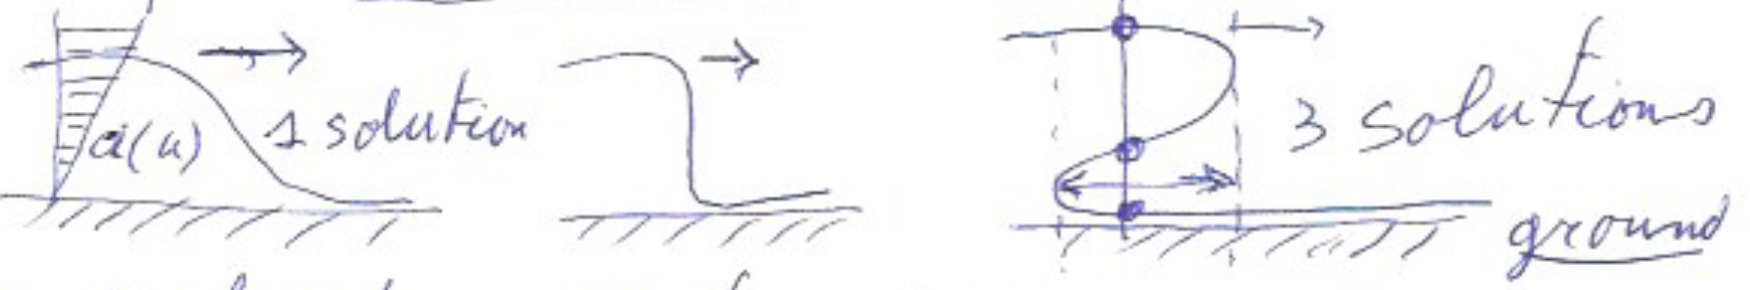
\includegraphics[scale=0.3]{ch8/13}
	\captionof{figure}{}
	\end{center}		
	
	This is due to the fact that the wave moves slower near the ground (ex: wave at the beach). But with Euler equations this is not permitted since the solution has to be unique and thus can be interpreted as a shock wave. 
	}
	
\subsection{Linear system of 2 first order PDE}
	This case corresponds to equations as: 
	
	\begin{equation}
	\frac{\D U}{\D x} + A \frac{\D U}{\D y} = 0 \qquad U = \left(\begin{array}{c}
	u\\
	v
	\end{array}
	\right)
\end{equation}			
	and A is a $4\times 4$ matrix. 
	
	\exemple{
	
	Consider the \textbf{second order D'Alembert wave equation}: 
	
	\begin{equation}
	\phi _{xx}-c^2 \phi _{yy} = 0
	\label{eq:dalembert}
\end{equation}		
	
	The solution of this equation is: 
	
	\begin{equation}
	\phi (x,y) = F_1(x-cx ) +  F_1(x + cx )
	\end{equation}
	where $F_1$ is the forward moving wave with speed +c and the backward for the other. There are 2 initial data to give, $F_1(y)$ and $F_2(y)$: $\phi (y,0) = F_1(y) + F_2(x)$. Let's solve \autoref{eq:dalembert} in a different way by defining: 
	
	\begin{equation}
	u = \phi _x, v = \phi _y \qquad \Rightarrow \begin{aligned}
	&u_x - c^2 v_y = 0 \\
	&v_x - u_y = 0
	\end{aligned}
	\end{equation}
	
	and in the matrix form: 
	
	\begin{equation}
	\frac{\D}{\D x} \left( 
	\begin{array}{c}
	u\\
	v	
	\end{array}
	\right)
	= 
	\left( 
	\begin{array}{cc}
	0 & -c^2\\
	-1 & 0	
	\end{array}
	\right)
	\frac{\D }{\D y}
	\left( 
	\begin{array}{c}
	u\\
	v	
	\end{array}
	\right)
	= 0
	\end{equation}
	
	\textbf{The eigenvalues of A are the wave speeds} $\bm{\pm c}$. Thus define the characteristic curves, here 2 families of curves. 
	
	\begin{center}
	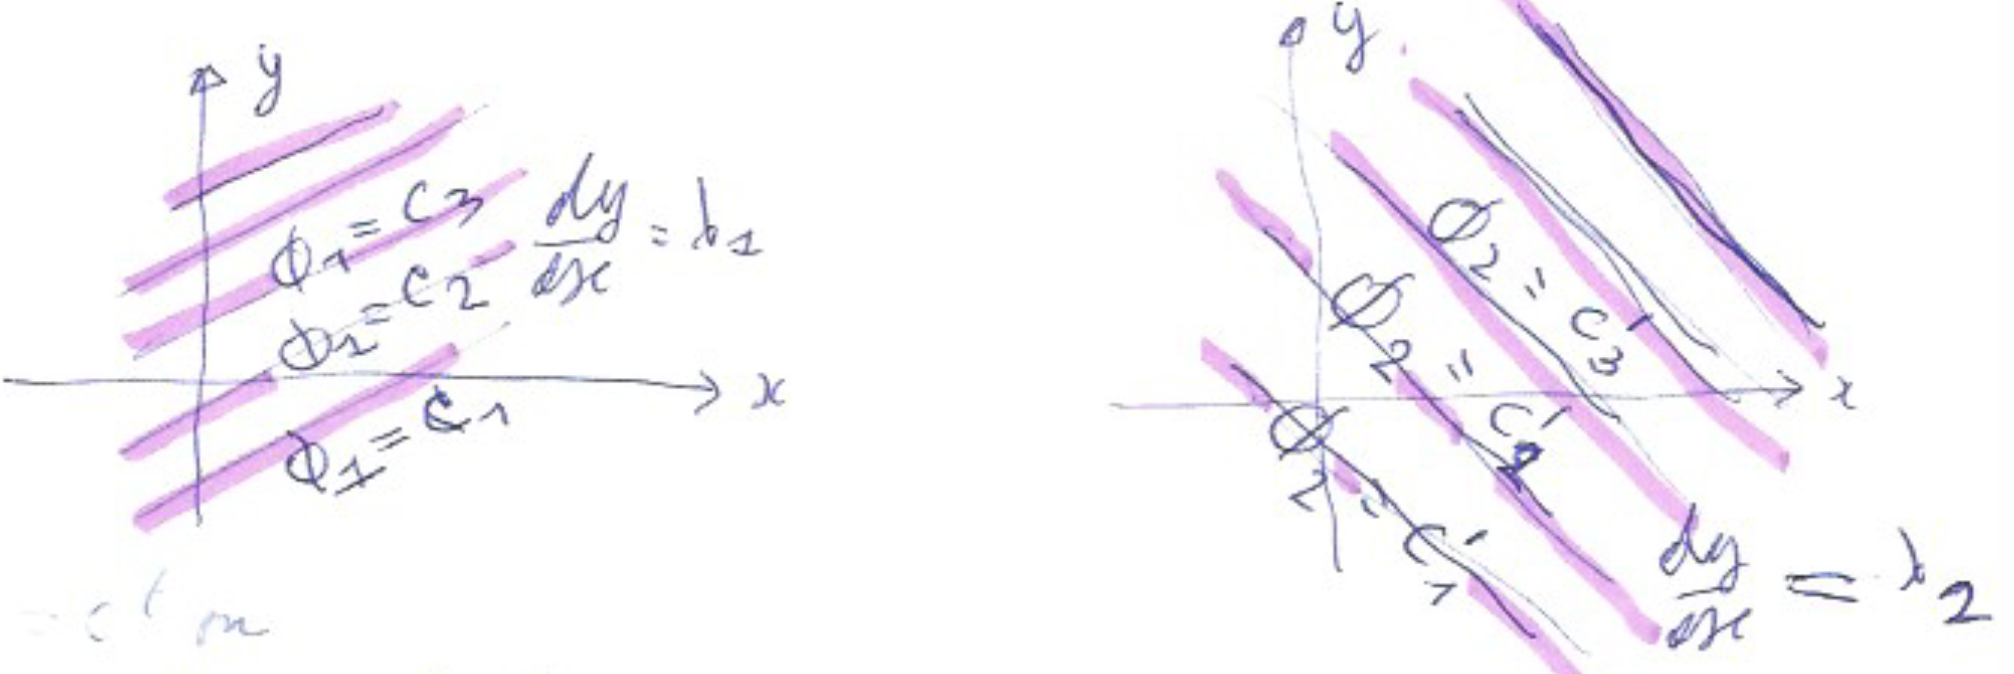
\includegraphics[scale=0.3]{ch8/14}
	\captionof{figure}{}
	\end{center}	 
	
	Hence the solution is: 
	
	\begin{equation}
	\phi (x,y) = \phi _1 (x,y) + \phi _2 (x,y) = F_1 (y-cx) + F_2 (y+cx)
	\end{equation}
	
	with $\phi _{1,2} (x,y) = F_{1,2} = cst$ on respectively family 1 and 2. Be careful that this only works if $\lambda_j (A) \in \mathcal{R}$, definition of hyperbolic system of PDE.
	}
	
	\exemple{
	Consider now the elliptic equation: 
	
	\begin{equation}
	\phi _{xx} + c^2 \phi _{yy} = 0
	\end{equation}
	
	For the same procedure as above, we obtain complex eigenvalues: $\lambda = \pm ic$. So if $\lambda _j (A)$ are complex with non zero imaginary part, the system is called \textbf{elliptic}.
	}
	
	\ \\ Note that for a 3rd order system (hybrid system), the eigenvalues can be 1 real + 2 complex conjugate or 3 real (hyperbolic). Elliptic is impossible. If 4th order, elliptic, thus \textbf{biharmonic}. 
	
	\exemple{
	Linearized potential flow: 
	
	\begin{equation}
	\phi _{yy} - \frac{1}{M^2_\infty - 1} \phi _{xx} = 0 
\end{equation}		

	For supersonic flows, we have hyperbolic wave equation and for subsonic we have an elliptic diffusion equation since we have $c^2 = \pm \frac{1}{M^2_\infty - 1} \Rightarrow \lambda _1^\pm = \pm c$ and $\lambda_2^\pm = \pm ic$. Below is represented the supersonic case. 
	
	\begin{center}
	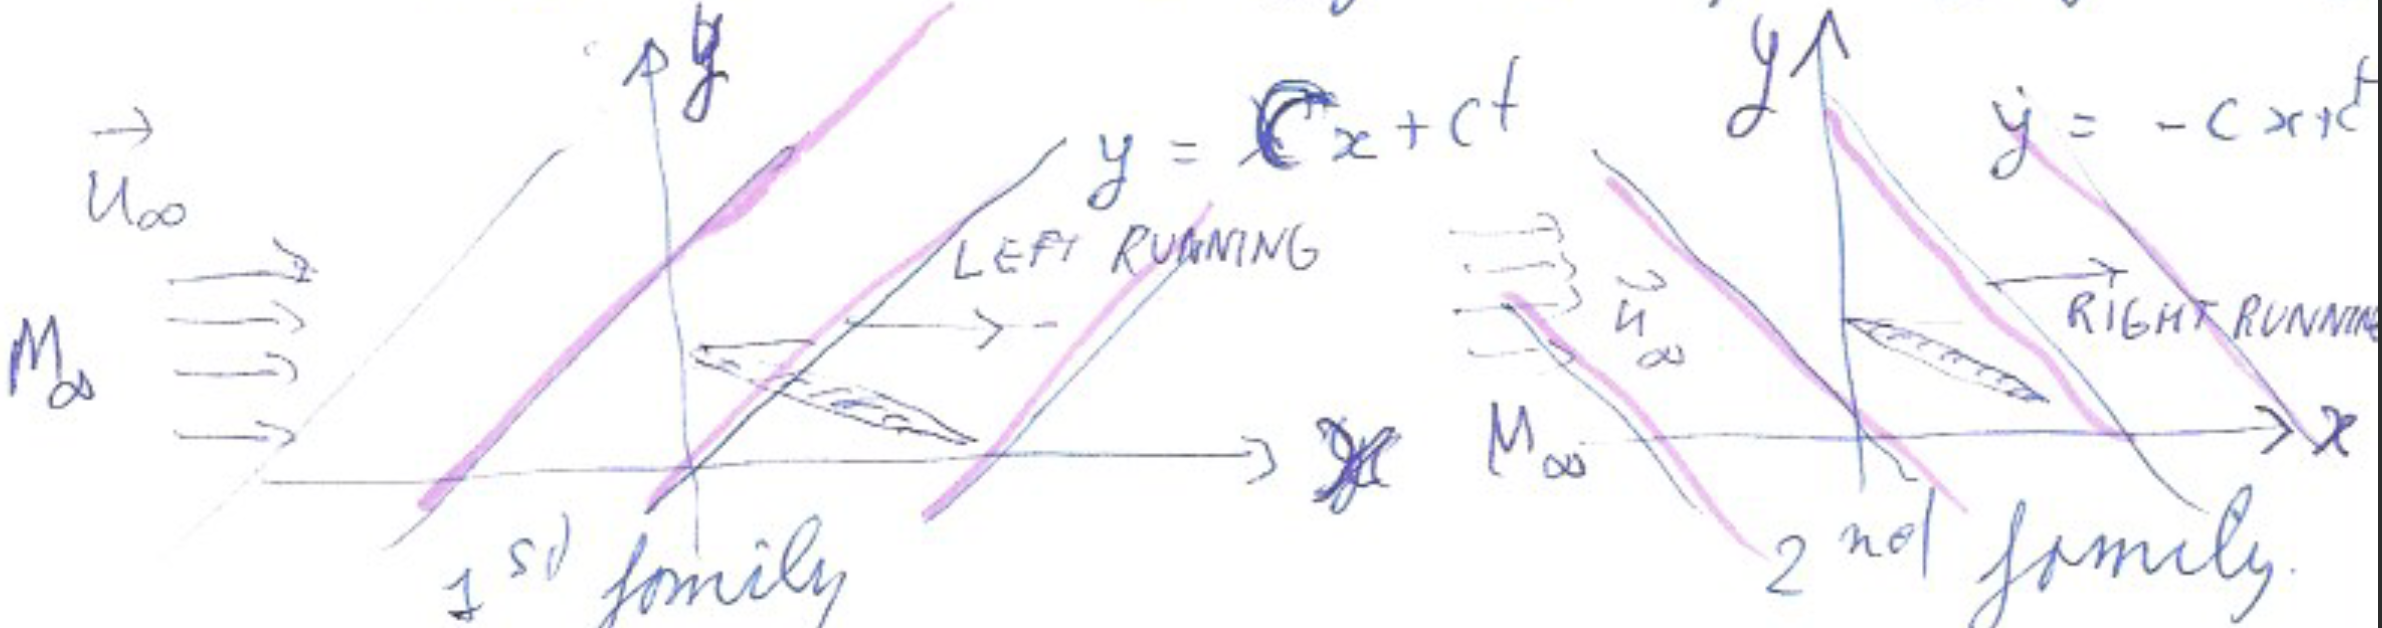
\includegraphics[scale=0.3]{ch8/15}
	\end{center}
	
	Depending on the initial conditions we are in 1 or 2, if $F_1(x) = 0$ first and same for the inverse. In this case the characteristic curves are called the \textbf{Mach lines} and $\tan \mu = \frac{1}{\sqrt{M^2_\infty - 1}}$
	}
	
\subsection{Method of characteristics for a 1st order system of PDE for constant coefficients}
	We intend to solve the hyperbolic equation: 
	
	\begin{equation}
	\frac{\D U}{\D x} + A \frac{\D U}{\D y} = 0
	\end{equation}
	
	The idea is to convert this to a decoupled system of 2 scalar wave equations by diagonalizing: 
	
	\begin{equation}
	LAR = D = \left( 
	\begin{array}{cc}
	\lambda _1 & 0\\
	0 & \lambda _2
	\end{array}
	\right) \qquad R = (r_1 \ r_2) \qquad L = (l_1 \ l_2) ^t
	\end{equation}
	
	where $r_i$ are column eigenvectors and $l_i$ row eigenvectors with $L = R^{-1}$. For this, we multiply the system of equation by L and we add RL since LR = I: 
	
	\begin{equation}
	L\frac{\D U}{\D x} + LARL \frac{\D U}{\D y} = 0 \quad \Rightarrow 	\frac{\D LU}{\D x} + LAR \frac{\D LU}{\D y} = 0
	\end{equation}
	
	and we define the \textbf{characteristic variables}: $W = LU = (w_1 \ w_2)^t$ ad we get the decoupled system: 
	
	\begin{equation}
	\frac{\D W}{\D x} + D \frac{\D W}{\D y} = 0
	\end{equation}
	
	The solution of the first and second are: 
	
	\begin{equation}
	\begin{aligned}
	w_1(x,y) = w(y- \lambda _1 x) \quad w_1(x,y) = cst \ on \ \frac{\d y}{dx} = \lambda _1\\
	w_2(x,y) = w(y+ \lambda _2 x) \quad w_2(x,y) = cst \ on \ \frac{\d y}{dx} = \lambda _2
	\end{aligned}
	\end{equation}
	
	\wrapfig{6}{l}{5}{0.3}{ch8/16}{ch8/16}
	The constant is fixed by the initial data on $x=0$: 
	\begin{equation}
	w_1(x_P, y_P) = w_1^* (x_A, y_A)\\
	w_2(x_P, y_P) = w_2^* (x_B, y_B)
	\end{equation}
	
	So to find the solution in P: 
	
	\begin{enumerate}
	\item Find the two characteristic curves
	\item Trace back to the initial data to find the constants
	\item Transform back to the variable U: 
	
	\begin{equation}
	U_P = RW_P
	\end{equation}
	\end{enumerate}
	
\subsubsection{Application to the potential flow}
	The characteristic curves are: 
	
	\begin{equation}
	C^\pm: \quad \left(\frac{dy}{dx}\right)^\pm = \pm \frac{1}{\sqrt{M^2_\infty -1}} = \tan (\pm \mu _\infty) 
	\end{equation}
	
	There are two ways of computing the eigenvectors: solving $AR = RD$  or $Ar_j = \lambda _jr_j $and $LA = DL$ or $l_jA = \lambda _jl_j $for $r_j$ and $l_j$ respectively, we prefer the second. In our case: 
	
	\begin{equation}
	l_1 A = \lambda _1 l_1 \qquad \Rightarrow (\alpha \ \beta) \left(
	\begin{array}{cc}
	0 & -c^2\\
	-1 & 0
	\end{array}
	\right)
	= +c (\alpha \beta)
	\end{equation}
	
	After solving we find: $l_1 = c^t(1 \ -c)$ and $l_2 = c^t(1 \ +c)$. The characteristic variable $W = LU$ is: 
	
	\begin{equation}
	\begin{aligned}
	w_1 = l_1 U = c^t (u  -\frac{1}{\sqrt{M_\infty^2 -1}} v)\\
	w_2 = l_2 U = c^t (u  +\frac{1}{\sqrt{M_\infty^2 -1}} v)
	\end{aligned}
	\end{equation}
	
	and these functions are constant along the characteristic curves and are called \textbf{Riemann invariant}. 
	
	\wrapfig{6}{l}{5}{0.3}{ch8/17}{ch8/17}
	Remember that u and v are the perturbation velocities. To compute them on the lower side of the profile we use $C^-$: 
	
	\begin{equation}
	u_P + \frac{v_P}{\sqrt{M^2_\infty -1}} = u_\infty + \frac{v_\infty}{\sqrt{M^2_\infty -1}} = 0 
	\end{equation}
	
	the second member is null since there is no perturbation at $\infty$. There are still the boundary conditions: 
	
	\begin{equation}
	\frac{v_P}{V_\infty + u_P}= \tan \theta _{wall} \qquad \Rightarrow \frac{v_P}{V_\infty} \approx \theta _{wall}
	\end{equation}
	
	So that we can find the velocities:
	
	\begin{equation}
	v^-_P = V_\infty \theta^- _{wall} \quad \Rightarrow u_P^- = \frac{V_\infty\theta ^-_{wall}}{\sqrt{M_\infty ^2 - 1}} \quad \Rightarrow c_P^- = \frac{-2 \theta ^-_{wall}}{\sqrt{M_\infty ^2 - 1}}
	\end{equation}
	
	Which is the previously seen \textbf{Ackaret's law}. Same process applied to the upper side gives the same results with inverted signs. \\
	
	For non-linear PDE's, the idea is exactly the same, the only difference is that the variable U will appear in the $\lambda$, the $L(U)$ and that the decoupled equations have the form: 
	
	\begin{equation}
	\frac{\D w_1}{\D x} + \lambda _1(U) \frac{\D w_1}{\D y} = 0 
	\end{equation}
	
	This is an ODE along the characteristic curve: $\frac{dw_1}{ds} = 0$ with $ds = \frac{\D}{\D x} + \lambda_1(U) \frac{\D}{\D y}$.
	
\subsection{Expansion waves}
	\wrapfig{7}{l}{6}{0.25}{ch8/6}{ch8/6}
	Consider in the figure the convention $d\theta < 0$. The infinitely small $d\theta$ induces an infinitely small perturbation noted $V+dV$. Since the Mach wave is also a solution of the flow equations, $V_t$ before and after the Mach wave is the same. We have: 
	
	\ \\
	
	\begin{equation}
	V_t = V\cos \mu = (V+dV) \cos (\mu - d\theta) \qquad \Leftrightarrow 1+\frac{dV}{V} = \frac{\cos \mu }{\cos (\mu - d\theta)}
	\end{equation}
	
	Using the fact that $d\theta$ is very small we get: 
	
	\begin{equation}
	1=\frac{dV}{V} \approx \frac{\cos \mu }{\cos \mu + d\theta \sin \mu } = 
	\end{equation}